\documentclass[12pt]{report}
\usepackage{fullpage}
\usepackage{amssymb}
\usepackage{amsmath}
\usepackage{enumitem}
\usepackage{graphicx}
\usepackage{float}
\usepackage[colorlinks,citecolor=DeepPink4,linkcolor=DarkRed‌​]{hyperref}
\usepackage{url}


\usepackage[utf8]{inputenc}
\usepackage{textcomp}
\usepackage{mathtools}
\usepackage{amsmath}
\usepackage{fancyhdr}
\pagestyle{fancy}
\fancyhf{} % clear all header and footer fields
\rfoot{https://github.com/afollestad/material-dialogs/issues/1162}
\renewcommand{\headrulewidth}{0pt}
\renewcommand{\footrulewidth}{0pt}

% each section on new page
\usepackage{etoolbox}
\pretocmd{\section}{%
  \ifnum\value{section}=0 \else\clearpage\fi
}{}{}




\renewcommand{\familydefault}{\sfdefault} % change font family to sans serif

\begin{document}

\title{Software Analytics - Bug details}
\author{Talal El Afchal}
\date{\today}
\maketitle
	\section*{Bug}
\href{https://github.com/afollestad/material-dialogs}{Material$-$dialogs} is an Android customizable dialogs API. The Git repository has 8758 $\star$ and 1440 commits.
The framework provides many types of dialog window, one of them is the \emph{Basic list} dialog which consists of a list of items and one check-box as shown in figure 1

\begin{figure}[H]
	\centering
	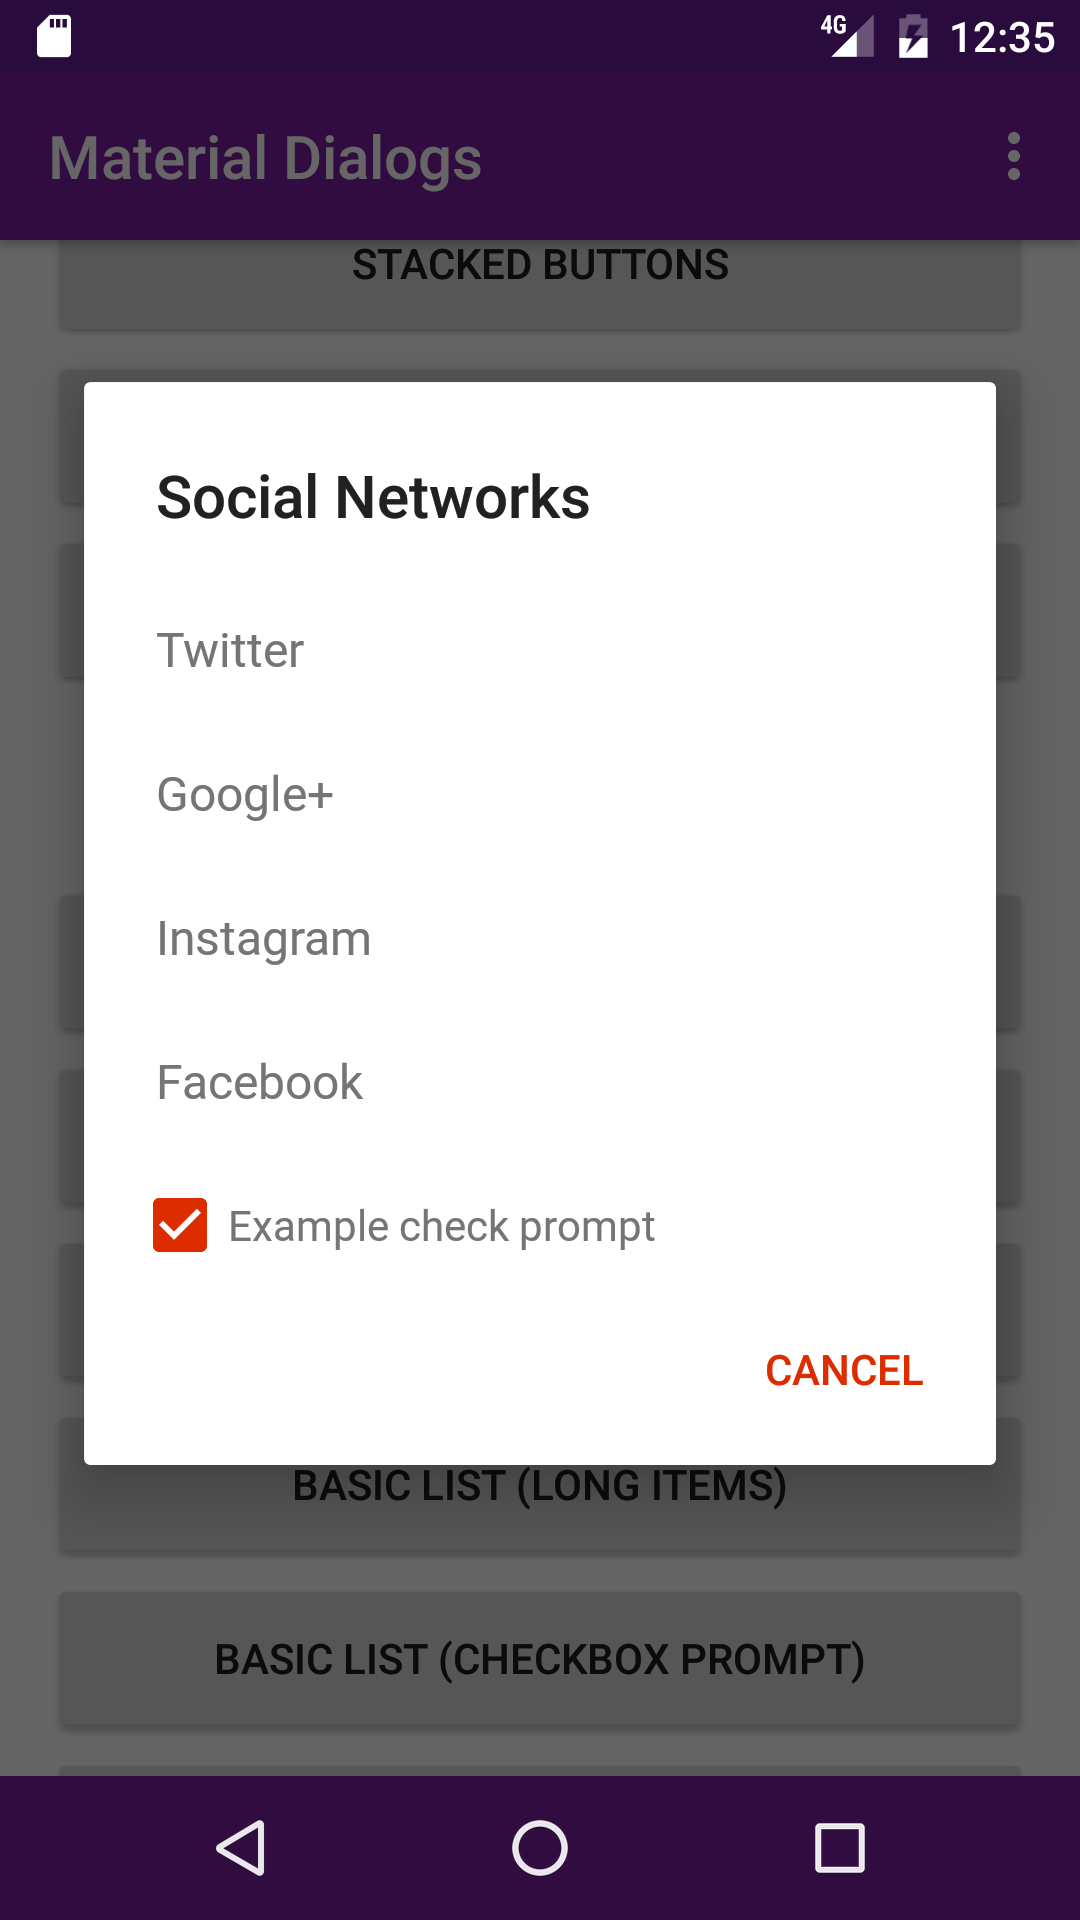
\includegraphics[height=0.4\textwidth]{screenshots/portrait.png}
	\caption{portrait}
\end{figure}
\noindent When the phone is in the landscape mode the check-box disappears as shown in figure 2, but the check-box must be visible like it is in the portrait mode.\\ On November 4, 2016 a \href{https://github.com/afollestad/material-dialogs/issues/1162}{\emph{``bug''}} label was added and on Jan 4, 2017 a \emph{``help wanted''} label was also added.\\


\begin{figure}[H]
	\centering
	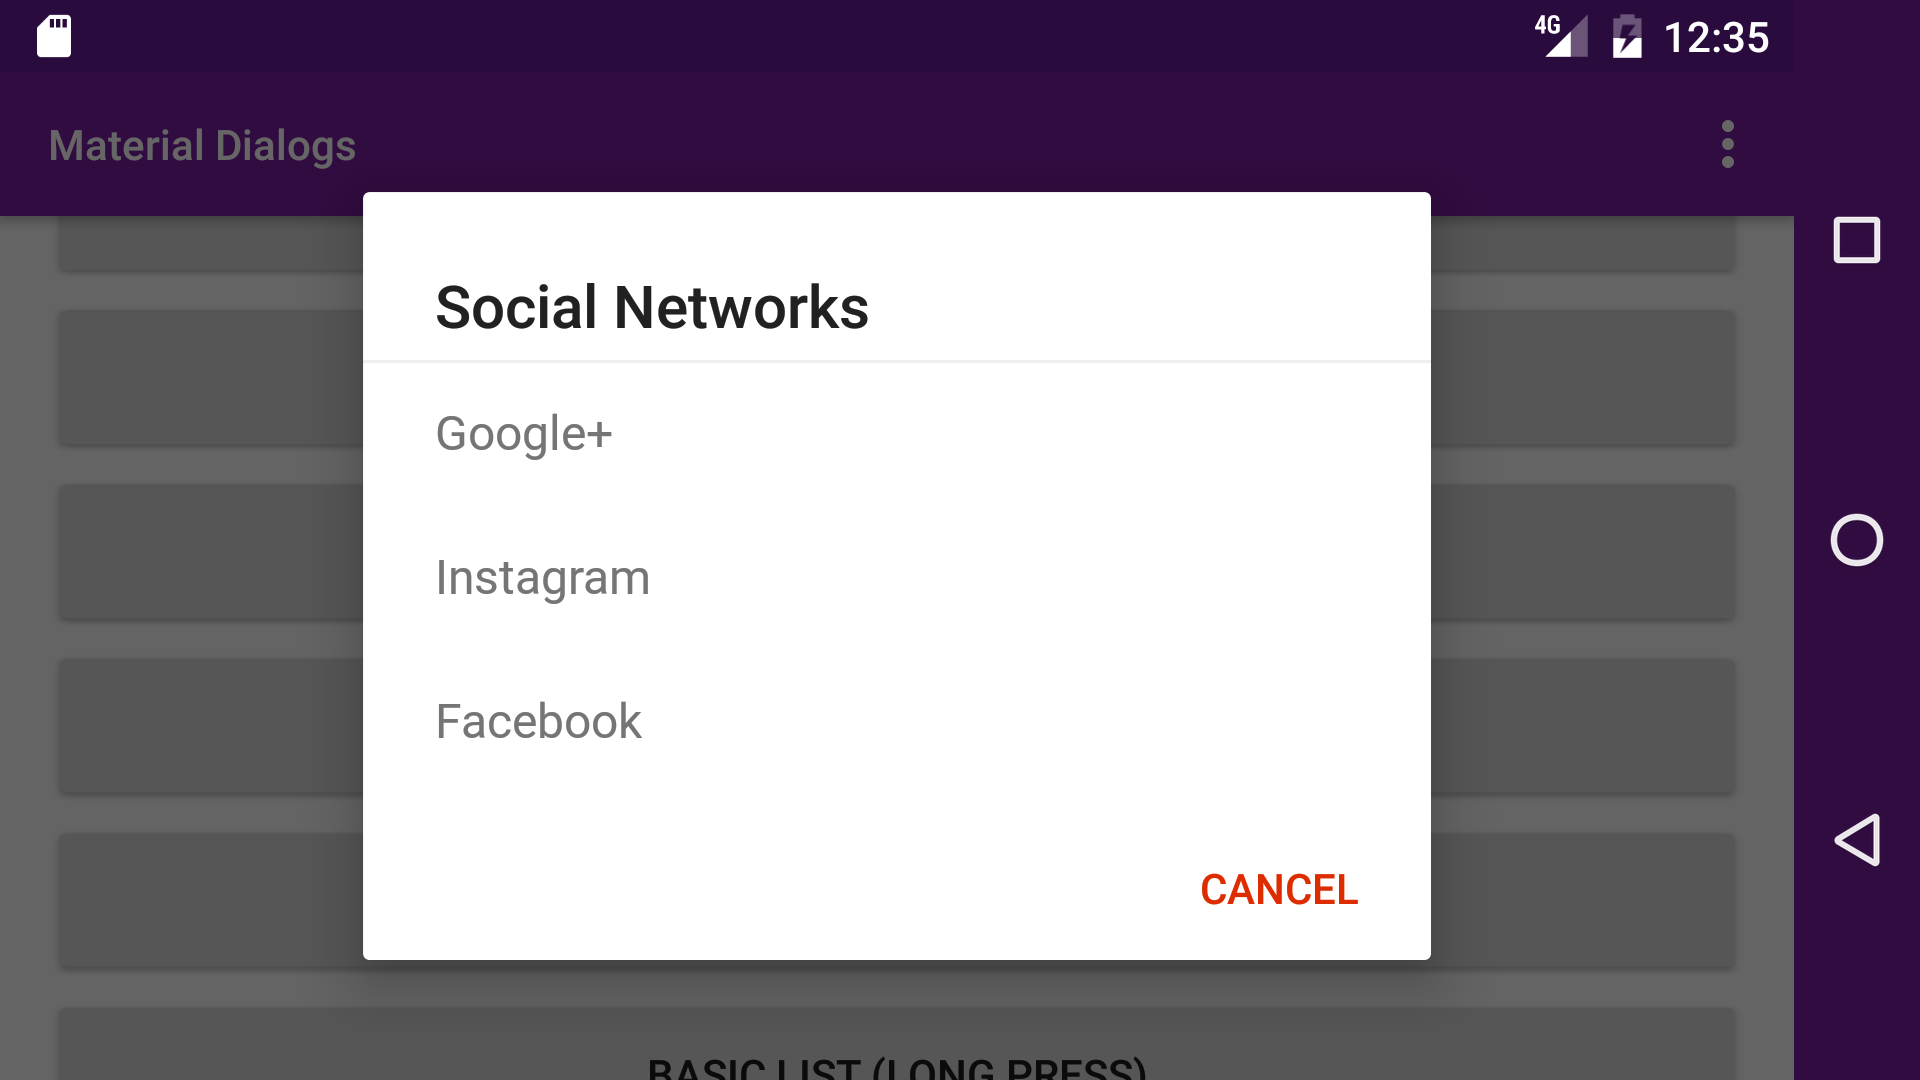
\includegraphics[width=0.6\textwidth]{screenshots/landscape.png}
	\caption{landscape}
\end{figure}



\end{document}








